\chapter{Introdução}

As Bolhas de Plasma Equatorial (\textit{Equatorial Plasma Bubbles} - EPB) são zonas caracterizadas por flutuações na densidade do plasma que se formam na ionosfera de baixa latitude, principalmente durante o período após o pôr do sol. Elas submetem os sinais de rádio a variabilidades de amplitude e de fase, afetando o funcionamento de sistemas tecnológicos que utilizam os sinais dos Sistemas Globais de Navegação por Satélite (GNSS) para navegação \cite{Githio2024}.

As EPBs apresentam morfologias características que podem ser identificadas em imagens de airglow, como mostrado na Figura \ref{fig:epb_temporal}, onde observam-se estruturas ramificadas e alongadas que se estendem verticalmente através da ionosfera e apresentam evolução temporal dinâmica.

A relevância do Brasil para a detecção, monitoramento e estudo das EPBs é extremamente alta, devido à sua localização geográfica e geomagnética única e ao papel ativo de suas instituições de pesquisa, como o Instituto Nacional de Pesquisas Espaciais (INPE), através do Programa de Estudo e Monitoramento Brasileiro de Clima Espacial (EMBRACE) cujo objetivo principal é monitorar, modelar e difundir informações sobre o Clima Espacial para prever e mitigar seus impactos sobre as atividades tecnológicas, econômicas e sociais no Brasil \cite{EMBRACE2021}.

Tradicionalmente, os eventos de EPBs são identificados principalmente pelo olho humano, um método demorado e ineficiente, facilmente influenciado pela subjetividade do observador e não é escalável para o volume de dados observacionais gerados atualmente. Por exemplo, um imageador airglow de canal único de uma única estação no Projeto Meridiano Chinês gera cerca de 1 TB de dados por ano, tornando o processamento manual um desafio significativo \cite{Zhong2025}.

Técnicas de aprendizado de máquina têm sido aplicadas para automação da detecção de EPBs. \citeonline{Thanakulketsarat2023} desenvolveram um modelo combinado de CNN/SVM com kernel RBF, alcançando acurácia de 93,67\%. \citeonline{Yacoub2025} propuseram uma abordagem utilizando Análise de Componentes Principais Bidimensional (2DPCA) para extração de características espaciais, combinada com \textit{Recursive Feature Elimination} (RFE) e classificador Random Forest, atingindo acurácia de 98,17\%. Embora promissores, estes estudos focaram principalmente em datasets específicos, havendo necessidade de adaptação às características particulares das imagens airglow brasileiras do programa EMBRACE/INPE.

Este projeto propõe o desenvolvimento de uma abordagem baseada em \textit{deep learning} para detecção automática de EPBs em imagens airglow do EMBRACE, explorando arquiteturas modernas de CNN adaptadas às características específicas dessas estruturas ionosféricas. A pesquisa situa-se na interseção entre ciências espaciais e inteligência artificial, contribuindo tanto para o avanço metodológico em visão computacional quanto para o aprimoramento dos sistemas operacionais de monitoramento de clima espacial no Brasil. Espera-se reduzir o tempo de detecção, aumentar a consistência histórica e fornecer base metodológica para aplicações preditivas subsequentes de clima espacial no Brasil.

\begin{figure}[htb]
    \centering
    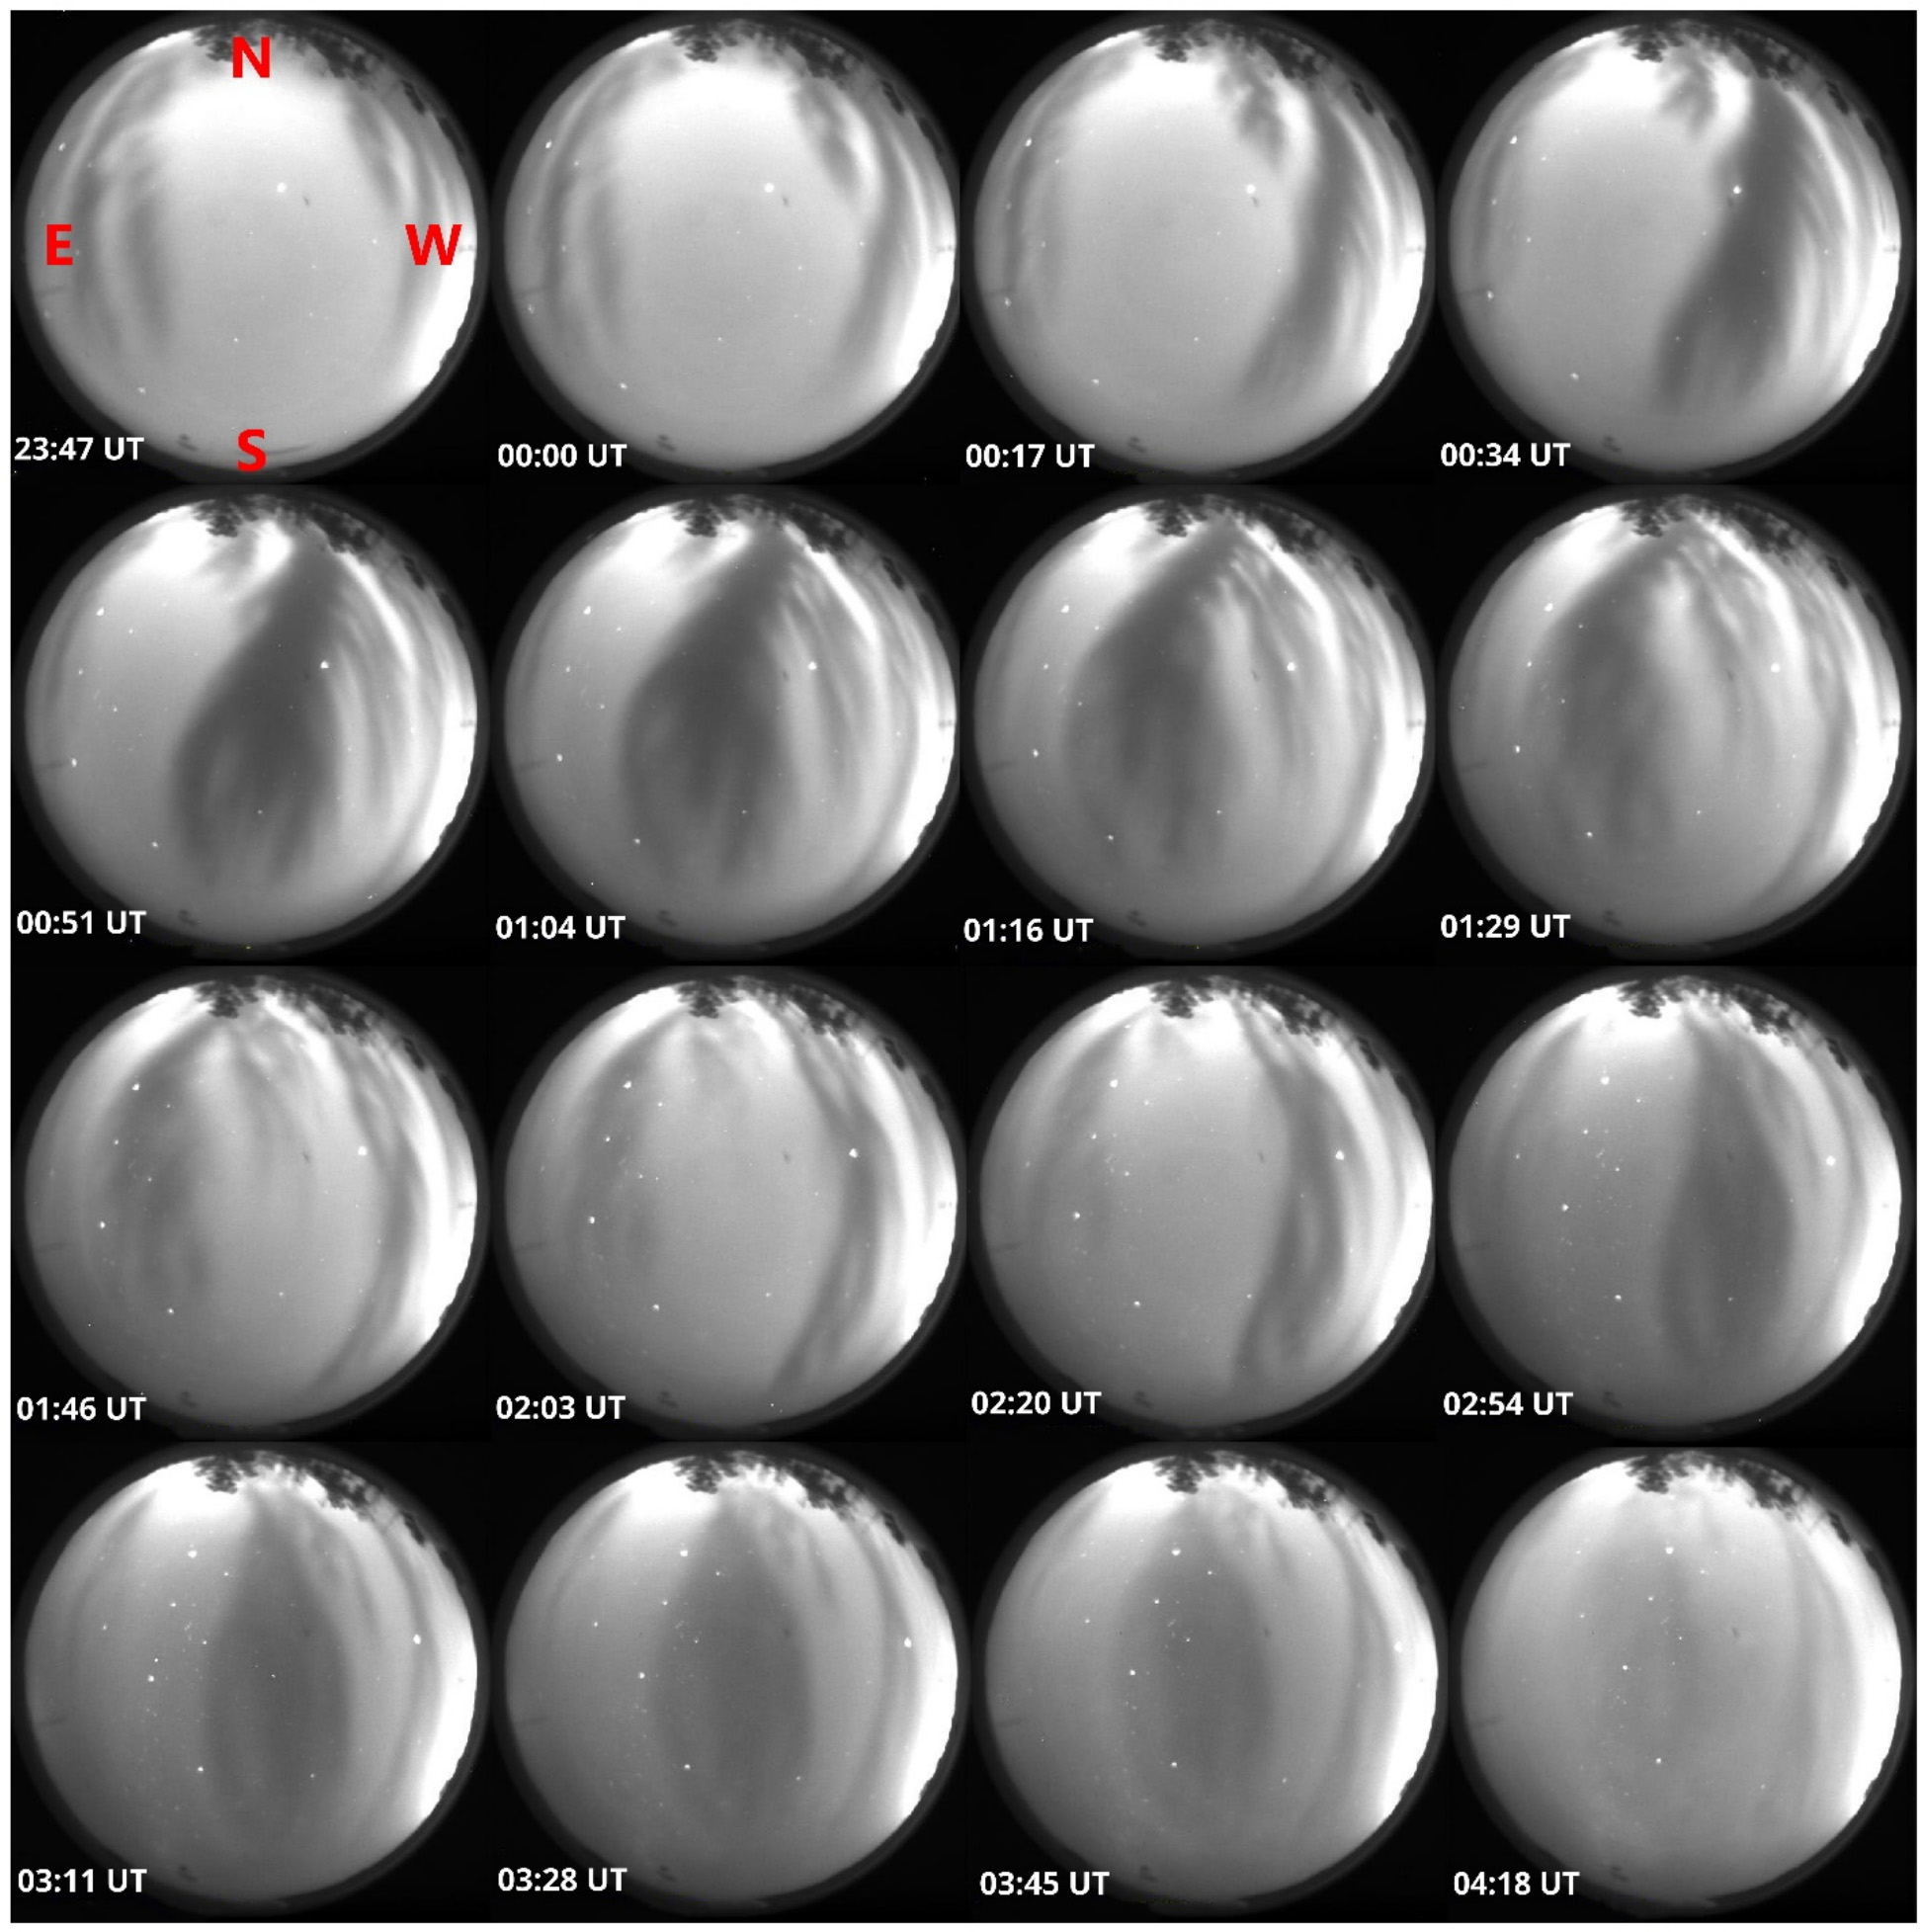
\includegraphics[width=0.9\textwidth]{epb.png}
    \caption[Sequência temporal de EPBs em airglow]{Sequência temporal de EPBs em imagens airglow (630{,}0 nm), 21/11/2022.}
    \fonte{Adaptado de \citeonline{Githio2024}.}
    \legend{\footnotesize Sequência de frames do imageador All-Sky (Cachoeira Paulista, DOY 325) mostrando estruturas ramificadas e alongadas (bandas escuras) que se deslocam para leste. A evolução evidencia a dinâmica das bolhas de plasma equatoriais e sua morfologia característica.}
    \label{fig:epb_temporal}
\end{figure}